\documentclass[12pt]{article}
\usepackage[margin=1in]{geometry}
\geometry{letterpaper}
\usepackage{graphicx}
\usepackage{amssymb}
\usepackage{epstopdf}
\DeclareGraphicsRule{.tif}{png}{.png}{`convert #1 `dirname #1`/`basename #1
.tif`.png}

\raggedright % So not straight on both sides
\setlength{\parindent}{0.5in} % So indent paragraphs
\usepackage{indentfirst} % So indent first paragraph after a heading
\usepackage{titlesec}
\usepackage{authblk}
\titleformat{\section}[block]{\normalsize \bfseries \filcenter}{}{1em}{}
\titleformat{\subsection}[block]{\normalsize \bfseries}{}{1em}{}
\titleformat{\subsubsection}[runin]{\bfseries}{}{}{}[]
\titlespacing{\subsubsection}{\parindent}{*2}{\wordsep}
\setcounter{secnumdepth}{0}
\usepackage{setspace}
\usepackage{apacite}
\usepackage{amsmath}
\usepackage{color} % So can change text colour, helpful for editting
\usepackage[usenames,dvipsnames,svgnames,table]{xcolor}
\usepackage{graphicx} % So can add pictures
\usepackage[labelfont=it, labelsep=period]{caption}
\usepackage{enumitem} % To format lists ok
\usepackage{booktabs, multirow, nameref}
% Pretty tables
\newcommand{\IE}[1][1]{% indent entry
  \hspace{#1em}\ignorespaces
}

\usepackage{array}
\newcolumntype{C}[1]{>{\centering\arraybackslash}m{#1}}
\newcolumntype{D}[1]{>{\footnotesize\let\newline\\\arraybackslash\hspace{0pt}}m{#1}}

% For Bayesian model diagram
\usepackage{tikz}
\usetikzlibrary{bayesnet}
% See https://github.com/jluttine/tikz-bayesnet

\usepackage{fancyhdr} % To add headers
\setlength{\headheight}{15.2pt}
\pagestyle{fancy}
\usepackage{lastpage}
\lhead[RECOGNITION \& CATEGORIZATION]{RECOGNITION \& CATEGORIZATION}


\title{Recognition performance after rule-based and information-integration
categorization.}
\author{C. E. R. Edmunds, Lenard Dome, Andy J. Wills \& Fraser Milton}

\begin{document}

\maketitle

\begin{abstract}
A large portion of the category learning literature is dedicated to discussing the stimulus representations underlying categorization. 
The SUSTAIN model has proved successful in accounting for categorization effects by proposing a middle ground between exemplar, prototype and rule representations. 
One exception to SUSTAIN's success may be in accounting for learning in information-integration tasks, which have been extensively argued to be learned implicitly (contrary to the predictions of SUSTAIN). 
However, recent work has failed to evidence for an implicit mechanism in this task. 
Therefore, in the following we investigated explicit recognition performance after learning either rule-based or information-integration tasks. 
We found that, contrary to the claims in the literature, that recognition memory was better following the information-integration task than the rule-based task and that this is predicted by the SUSTAIN model. 
Our results add to the growing literature that suggests that both of these categorization tasks are learned explicitly. 
\end{abstract}
\newpage

\doublespacing

The category learning literature is abundant with formal models, all making disparate assumptions about stimulus representation, generalization, grouping and decision-making \cite{Pothos2011}. 
One of these, the SUSTAIN model \cite<Supervised and Unsupervised STratified Adaptive Incremental Network;>{Love2004}, accounts for an impressive variety of categorization phenomena: learning rates \cite{Love1998a}; superior recognition memory for exception items \cite{Davis2012a}; identification \cite{Love1998}; inference learning \cite{Love2000}; developmental categorization trajectories \cite{Gureckis2004}; and unsupervised learning \cite{Gureckis2002, Gureckis2003}. 
This breadth is particularly admirable given modelers' tendency to focus on a small subset of effects \cite{Wills:2017ez}. 

One area has been firmly placed outside the explanatory scope of SUSTAIN is procedural learning \cite{Davis2012a}.
The category representations formed by SUSTAIN and by procedural learning mechanisms are fundamentally different. 
SUSTAIN represents category structures using clusters of stimuli \cite{Love2004}, where each category might be represented by one or many clusters. 
In contrast, procedural learning proceeds incrementally \cite{Ashby1998}: visual inputs are gradually associated with a particular motor response using reward prediction error to moderate the weights. 
Thus, the response acts as a proxy for the category label: there is no intermediate generalisation stage. 
These contrasting approaches mean that SUSTAIN predicts very different behaviour to that observed in tasks optimally learned by a procedural mechanism. 

In the current work, we will consider a particular task widely argued to be learned procedurally: the information-integration (II) category structure \cite<see Figure~\ref{fig:categoryStructures}>{Ashby:2018gv}.
Optimal performance on an II task is argued to require participants to combine (at least) two independent, non-commensurate stimulus dimensions at a pre-decisional stage \cite{Ashby1998}. 
As the optimal decision is difficult to describe in this task\footnote{One contorted way of describing Figure~\ref{fig:categoryStructures} might be ``If the stimulus is darker than it is large, it is in Category A.''} many have argued that II tasks are learned procedurally \cite<for reviews, see>{Ashby2005c, Ashby2011b, Ashby:2017fm, Ashby:2018gv, Smith2018}. 

\begin{figure}[b!]
    \centering
    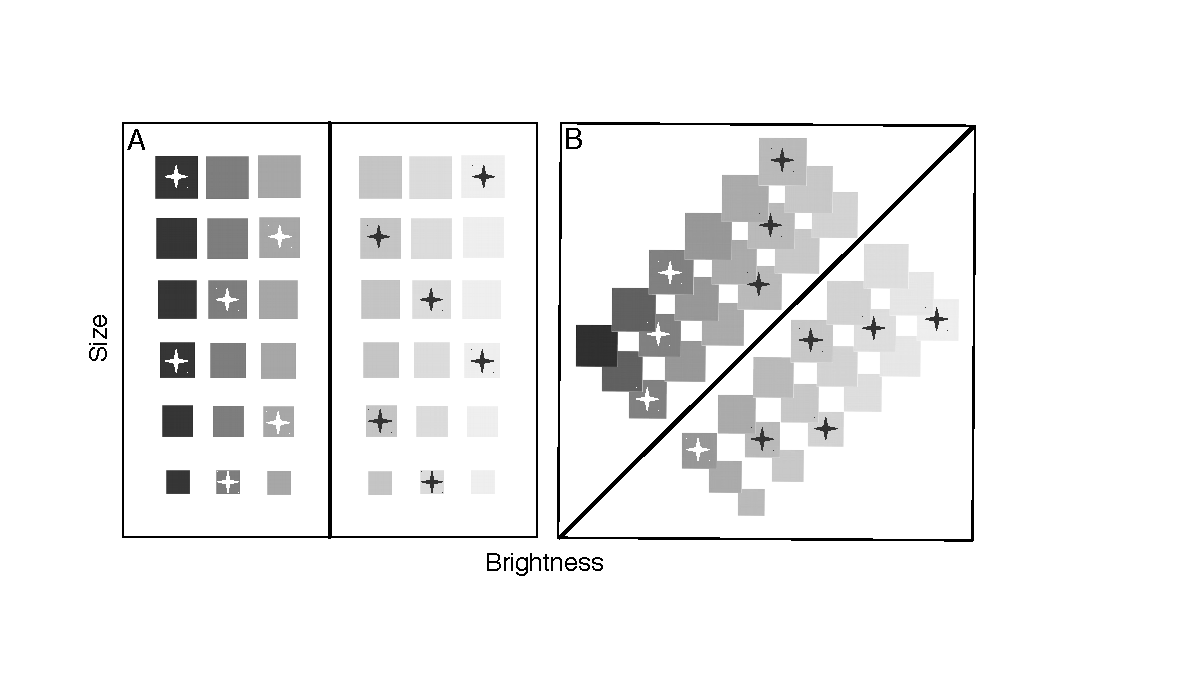
\includegraphics[width=0.8\textwidth]{Images/categoryStructures}
    \caption{Representations of the category structures used in the following experiments. Left: Unidimensional rule-based, Right: Information-integration. The
stars (colour irrelevant, not shown to the participants) mark a possible pattern of stimuli that were removed during the training phase of the experiment.}
    \label{fig:categoryStructures}
\end{figure}

The research often cited in support of the claim that II tasks are learned procedurally are studies that manipulate factors widely thought to affect procedural learning mechanisms. 
For instance, as prediction error is critical to this process, procedural learning mechanisms are thought to be sensitive to the nature and timing of feedback \cite{Ashby1998, Ashby2005c, Ashby2011b}.
In agreement with this, learning of II tasks is poorer when feedback is absent \cite{Ashby1999}, or delayed \cite{Maddox2003, Maddox2004}, or deferred \cite{Smith2014}. 
It is improved when more detailed feedback is given \cite{Ashby2007} and there is an opportunity for error prediction \cite{Ashby2002a}. 
%Similarly, the knowledge gained via procedural learning mechanisms are thought to be stimulus and motor response specific. 
%For instance, learning of an II task is reduced if the response keys for each category are switched \cite{Ashby2003}. 
In contrast, SUSTAIN is much less sensitive to the type and format of feedback as it can account for unsupervised category learning, where there is no feedback at all \cite{Gureckis2002, Gureckis2003}.

A further difference between procedural learning mechanisms and SUSTAIN is that they differ in their predictions about explicit knowledge or awareness of the information learned. 
SUSTAIN does not claim to learn implicitly. 
Further, it makes detailed predictions about explicit recognition memory performance following learning. 
In contrast, many have argued that the results of a procedural learning mechanism are not accessible to consciousness \cite<e.g.,>{Smith2014, Smith2015a}. 
Therefore, in the following we explore recognition performance following category learning to determine whether a cluster-based approach can successfully learn II category structures. 

%% LD 09-04-2020: SUSTAIN can do it by simply increasing the tau (threshold for recruiting clusters)
%% but maybe it should be modelled
%% CE: Sure you're right, but gonna stick to what the people who came up with the model said. Mainly, because otherwise what is the point of the paper? If you feel strongly about it we can stuff something in the discussion :) 
%% LD: Fair point. They didn't consider a lot of things. I was really just nit-picking. :)

The rest of the paper proceeds as follows. 
First, we use formal modelling to specify what SUSTAIN would predict for recognition performance following category learning. 
We take this formal modelling step as skipping it would remove one of the great benefits of formal models \cite{Wills2012, Wills:2017ez}. 
Further, we have previously found that the verbal descriptions associated with formal models often imply conclusions or patterns of data that are subsequently falsified. 
For instance, we found that a model that have been extensively argued to be able to optimally learn overall similarity structures (such as the II task) actually struggled. 
Specifically, we looked to see whether the implicit Procedural learning mechanism from the COVIS model \cite{Ashby1998} could learn an overall similarity structure \cite{Edmunds2016}. 
We found that without extensive changes to the model, the learning violated a key experimental feature: without changes, the learning curve was not monotonic. 
Therefore, in the following we looked to see whether SUSTAIN could learn the information-integration category structure. 
Second, we describe four experiments in which we investigated subsequent recognition performance following category learning of II category structures. 
We then use Bayesian modelling approaches to combine the results of these four studies, in order to better estimate whether recognition performance is improved or not. 
Finally, we discuss the implications of our findings. 

\section{SUSTAIN}
Here, we describe the process of generating predictions from the SUSTAIN model for the learning and recognition of UD and II category structures. 
To begin, we describe the approximation of the formal architecture of SUSTAIN.
Note that SUSTAIN is designed to incorporate both supervised and unsupervised learning but, given the nature of the task, here we only discuss supervised learning.
Then, we describe the abstract category structures and the model fitting process. 
Finally, we describe how we generated predictions from the model as well as highlighting the key features of these predictions. 

So, the SUSTAIN model. 
For a more detailed description of the formal model, we refer the reader to \citeA{Love2004}. 
Broadly, SUSTAIN learns category structures by assigning stimuli to clusters. 
The first cluster SUSTAIN creates is always centred on the first stimuli representation fed to the model.
Thus, the category structures are represented in two levels: a single category can be represented by one or many clusters with each cluster containing one or many stimuli. 
SUSTAIN aims for the simplest possible solution - typically sorting stimuli on the basis of a single dimension.
If a simple solution is not adequate, SUSTAIN adds more clusters as needed. 
This adaptiveness allows SUSTAIN to account for both rule-based and exemplar-based learning in a single framework. 

Now looking more closely at the mechanism of the model on a trial-by-trial basis. 
Given a new stimulus, the model compares it to the features of all existing clusters.
Similarity is defined as the distance between stimulus and cluster representations.
Each cluster activates based on its similarity to the stimulus weighted by attention.
This means that each dimension is differentially impactful in this stimulus-cluster comparison.
Higher activations will belong to clusters, which are the most similar to the stimulus representation. 

These activations will eventually compete to respond to the stimulus.
If there are many competing alternatives, clusters will have lower output 
values after competition - the model will be less confident in the
choice. 
SUSTAIN selects the cluster with the highest output value and uses it to
calculate the probability of making a response. 
It then updates the winning cluster to be more similar to the stimulus.

SUSTAIN only recruits a new cluster after a surprising event. In supervised
learning, the model expands its architecture in response to a prediction error.
If there is no surprising event, the model clusters together similar items. In
unsupervised learning, the model recruits clusters when the stimulus mismatches
existing clusters.

%% LD 09-04-2020: This is only true if the learning is unsupervised
% If the stimulus is sufficiently similar to a particular cluster, it joins that cluster.
% If the stimulus is not sufficiently similar to any clusters, a new cluster is formed for that stimulus. 

\subsection{Recognition in SUSTAIN}

The model was also supplemented to account for recognition performance 
of amnesic patients, infants, young adults, and older adults \cite{Love2007}. 
This was the addition of recognition scores, 
which were essentially the sum of output activations for all clusters \cite<Equation A6 in>{Love2007}.
The smaller the cluster, the greater the recognition memory associated with that cluster \cite{Davis2012a}.
So the higher the activation score is, the better the recognition of an item will be.

For example, let us assume that SUSTAIN recruits one cluster that captures 
large sets of stimuli within category. This will produce lower recognition scores overall,
because most stimuli will be further away from the prototypical cluster. But this will
also produce higher recognition scores for a small subset of stimuli happen
to be closer to the prototypical cluster.

On the other hand, SUSTAIN can also recruit many clusters that captures
small sets of stimuli within category. This will produce higher recognition scores
overall, because most stimuli will be close to its representative (exemplar) cluster.
Interestingly, this suggests that more complex problems will result in better recognition,
because SUSTAIN will recruit multiple clusters for each category.

The formal description of this recognition mechanism have its limitations. 
SUSTAIN mathematically specifies recognition scores after lateral inhibition
has taken place. It will only suffice for small number of clusters. If the model
recruits large number of clusters with a relatively low cluster competition 
parameter, the output activation scores \cite<Equation 6>{Love2004}
will be inhibited. This represents the idea that many competing alternatives
will reduce the confidence in the choice. So their sum will also be smaller
compared to having two clusters with high cluster competition parameter.
This contradicts to the way SUSTAIN incorporates recognition outlined above.

We decided to remedy this discrepancy between the theory and the exact,
formal specification of the mechanism in two steps. First, we decided to
sum activation scores before lateral inhibition takes place. This ensures
that it reflects the model's overall familiarity with the stimulus and
not its confidence. Second, we applied Shannon Entropy to the set of 
retrieved cluster activations. Shannon Entropy is a well-established
way to quantify the information content of any stochastic random variable 
set. This represent the idea, that you encode and can retrieve more
information by recruiting many exemplar clusters than creating one prototypical
cluster. The more clusters are active, the more information you retrieve
from memory. This recognition entropy, $R_{e}$, is specified as:
\begin{equation}
R_{e} = -\sum^n_{i = 1}{\Pr(H^{act}_j) \times \log_2{\Pr(H^{act}_j)}}
\end{equation}
where $n$ is the number of clusters stored in SUSTAIN. $H^{act}_j$ is the 
activation of $j$ cluster as output by Equation 5 in \citeA{Love2004}.
$\Pr(H^{act}_j)$ is the probability of $j$ cluster. The probabilities
are calculated by dividing the activation of cluster $j$ with the sum of
$n$ cluster activations. When $R_e$ is high, cluster retrieval results in more
information available to make a recognition judgement. When $R_e$ is low,
cluster retrieval results in less information, so you are more likely to
judge an item to be old or don't recognize an item. We are interested in
overall performance. So a simple descriptive statistic of the trial-by-trial
$R_e$ will be sufficient for our current endeavour. But it is possible to map 
$R_e$ to a choice axiom, where the model must judge whether it has seen the
stimulus before or not.

\subsection{Model fitting}
To examine the performance of the SUSTAIN model in UD and II tasks, we used the \texttt{catlearn} package \cite{catlearn} implemented in R \cite{Rcore}. 
This package includes implementations of prominent category and associative learning models along with canonical datasets \cite{Wills:2017ez}. 

In the following reported simulations, we had two aims: to show that SUSTAIN could indeed learn both UD and II tasks, and to find a measure that might discriminate learning between UD and II tasks. 
To start, we determined the parameters that would result in SUSTAIN best predicting the category labels from the stimuli for both the UD and II tasks. 
The category structures we used are shown in Figure~\ref{fig:categoryStructures}.
In addition, we also fitted SUSTAIN to the counterbalanced version of these category structures corresponding to a $\pi/2$ rotation. 
For the UD structure, this is where the decision boundary would discriminate based on size not brightness. 
For the II structure, the decision boundary has a negative slope rather than a positive one. 
We assumed that each stimulus would have been shown to participants 10 times each, resulting in 360 trials for each categorization task. 

The model was fitted to these category structures using a differential evolution algorithm, as implemented in the \texttt{DEoptim} package \cite{DEoptim} with the default strategy that minimized the negative log-likelihood.
The parameter search was limited according to the upper limits given in Table~\ref{table:SUSTAINparameterValues}. 
This was to encourage the parameter values to be similar to previous simulations \cite<e.g.>{Love2004}. 
We systematically varied the parameter $c$ which controls the speed of crossover adaptation in the differential evolution algorithm to find the value that resulted in the best fit. 

\begin{table}[t!]
	\centering
	\caption{SUSTAIN parameter values, fitted to the category structures.}
	\label{table:SUSTAINparameterValues}
	\begin{tabular}{l c c c c c}
	\toprule
	Parameters & Upper Limit & \multicolumn{4}{c}{Category structures}\\
               & & $UD^{length}$ & $UD^{orientation}$ & $II^{positive}$ & $II^{negative}$ \\
	\midrule
	
    Attentional focus $r$       & 20 & 20.0 & 20.0 & 11.523890 & 0.000004467 \\
    Cluster competition $\beta$ & 20 & 20.0 & 20.0 & 20.0        & 20.0 \\
    Decision constancy $d$      & 20 & 20.0 & 15.09278 & 20.0 & 20.0 \\
    Learning rate $\eta$        & 1  & 0.08772490 & 0.12087377 & 0.08579475 & 0.08739468 \\
	
	\bottomrule
	\end{tabular}
\end{table}
% The upper limits are not the same in the table as in the code. I can't remember which one is correct. 
% LD: I selected parameters that will be more similar to that of Love et al 2004
% I also realised that we don't know the upper bounds of those parameters.
% Some can go quite high, while others have to be constrained because of the
% limtations of R.

\subsection{Predictions}
To generate predictions, for each category structure, we used the best-fitting parameters to simulate the responses to 360 trials for 30 hypothetical participants. 
Each participant received trials in a random order. 
In Figure~\ref{fig:SUSTAINlearningCurveGraph} we can see that SUSTAIN can easily learn the category structures. 
Note that these accuracies are much higher than are typically found in learning these category structures, especially for the II task. 
This is due to the lack of noise as we were fitting the category structure, not data from real participants. 
% I could fit the participant data? 

\begin{figure}
	\centering
	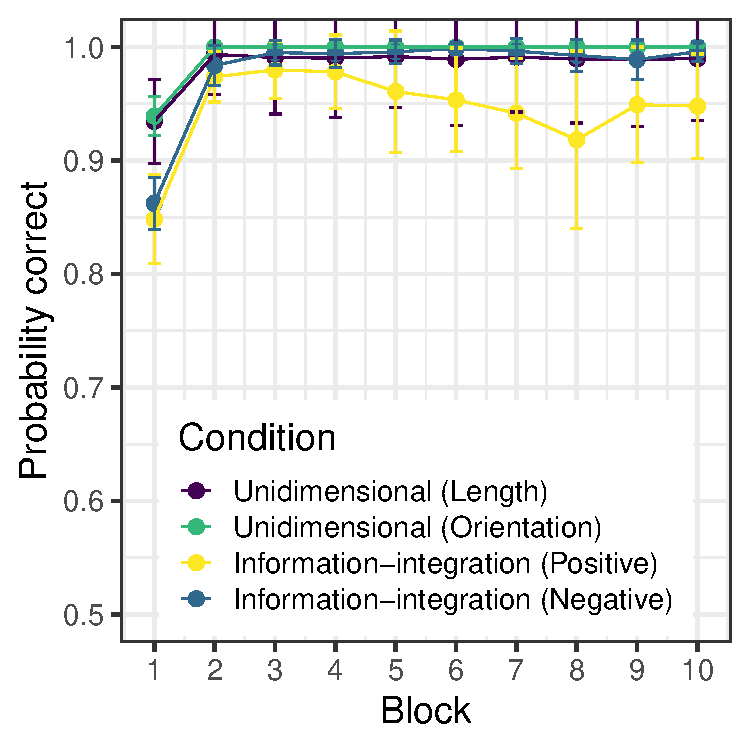
\includegraphics[width=0.5\textwidth]{Images/pu037learningCurveSUSTAIN}	
	\caption{Learning curve graphs for the UD and II category structures predicted by SUSTAIN}
	\label{fig:SUSTAINlearningCurveGraph}
\end{figure}

In all conditions, SUSTAIN exhibits a variety of solutions. The average 
number of clusters in the II tasks are higher
$M_\text{Positive}=16.80$, $SD=8.31$, $M_\text{Negative}=5.77$, $SD=0.89$,
than those in the UD tasks, $M_\text{Length}=3.30$, $SD=6.56$, $M_\text{Orientation}=2.23$, $SD=0.50$.

In Figure~\ref{fig:SUSTAINclusters} we show some examples of the clusters that SUSTAIN uses to learn these category structures. 
For the UD tasks, the simplest mapping from stimuli to clusters are a cluster per category. 
The most complex mapping has four clusters to a category structure $UD^{orientation}$. 
On the other hand, SUSTAIN can present an unexpected, more exemplar-like, behaviour 
under some cases. For examnple, in the $UD^{length}$ conditon, SUSTAIN recruits 
2 clusters for 26 simulated participants, and 3 clusters for 3 other simulated participants.
Simulation for one participant in the $UD^{length}$ condition resulted in the model recruiting
38 clusters. This number is higher than the number of stimuli in our simulation,
but organised along the grid-like arrangement of those stimuli. 

SUSTAIN is highly sensitive to trial-order effects \cite{Love2004} and this can result in
some unexpected behaviour. SUSTAIN adjusts the position of the winning cluster, so the 
cluster will become more prototypical and drift away from stimuli that it already captured 
once. If the model doesn't encounter the stimulus for many trials, the stimuli will become
more similar to other clusters. In that case, the model might be able to select the
wrong cluster mapped to the wrong category, even though it already knows the right response.
Then SUSTAIN would recruit a cluster in response to prediction errors. In response to prediction
error, the modal solution would be to adjust the closest cluster mapped to the right category
instead of recruiting a new category. We consider it to be the limitation of SUSTAIN, which
is only present in edge cases.

For the II task, the simplest mapping involves four clusters per category.
More complex clustering in this task becomes less ordered. Although it is 
definitely possible for SUSTAIN to learn both of these category structures,
the II task is generally more complex.

% LD: the colours are fairly hard to distinguish
\begin{figure}
	\centering
	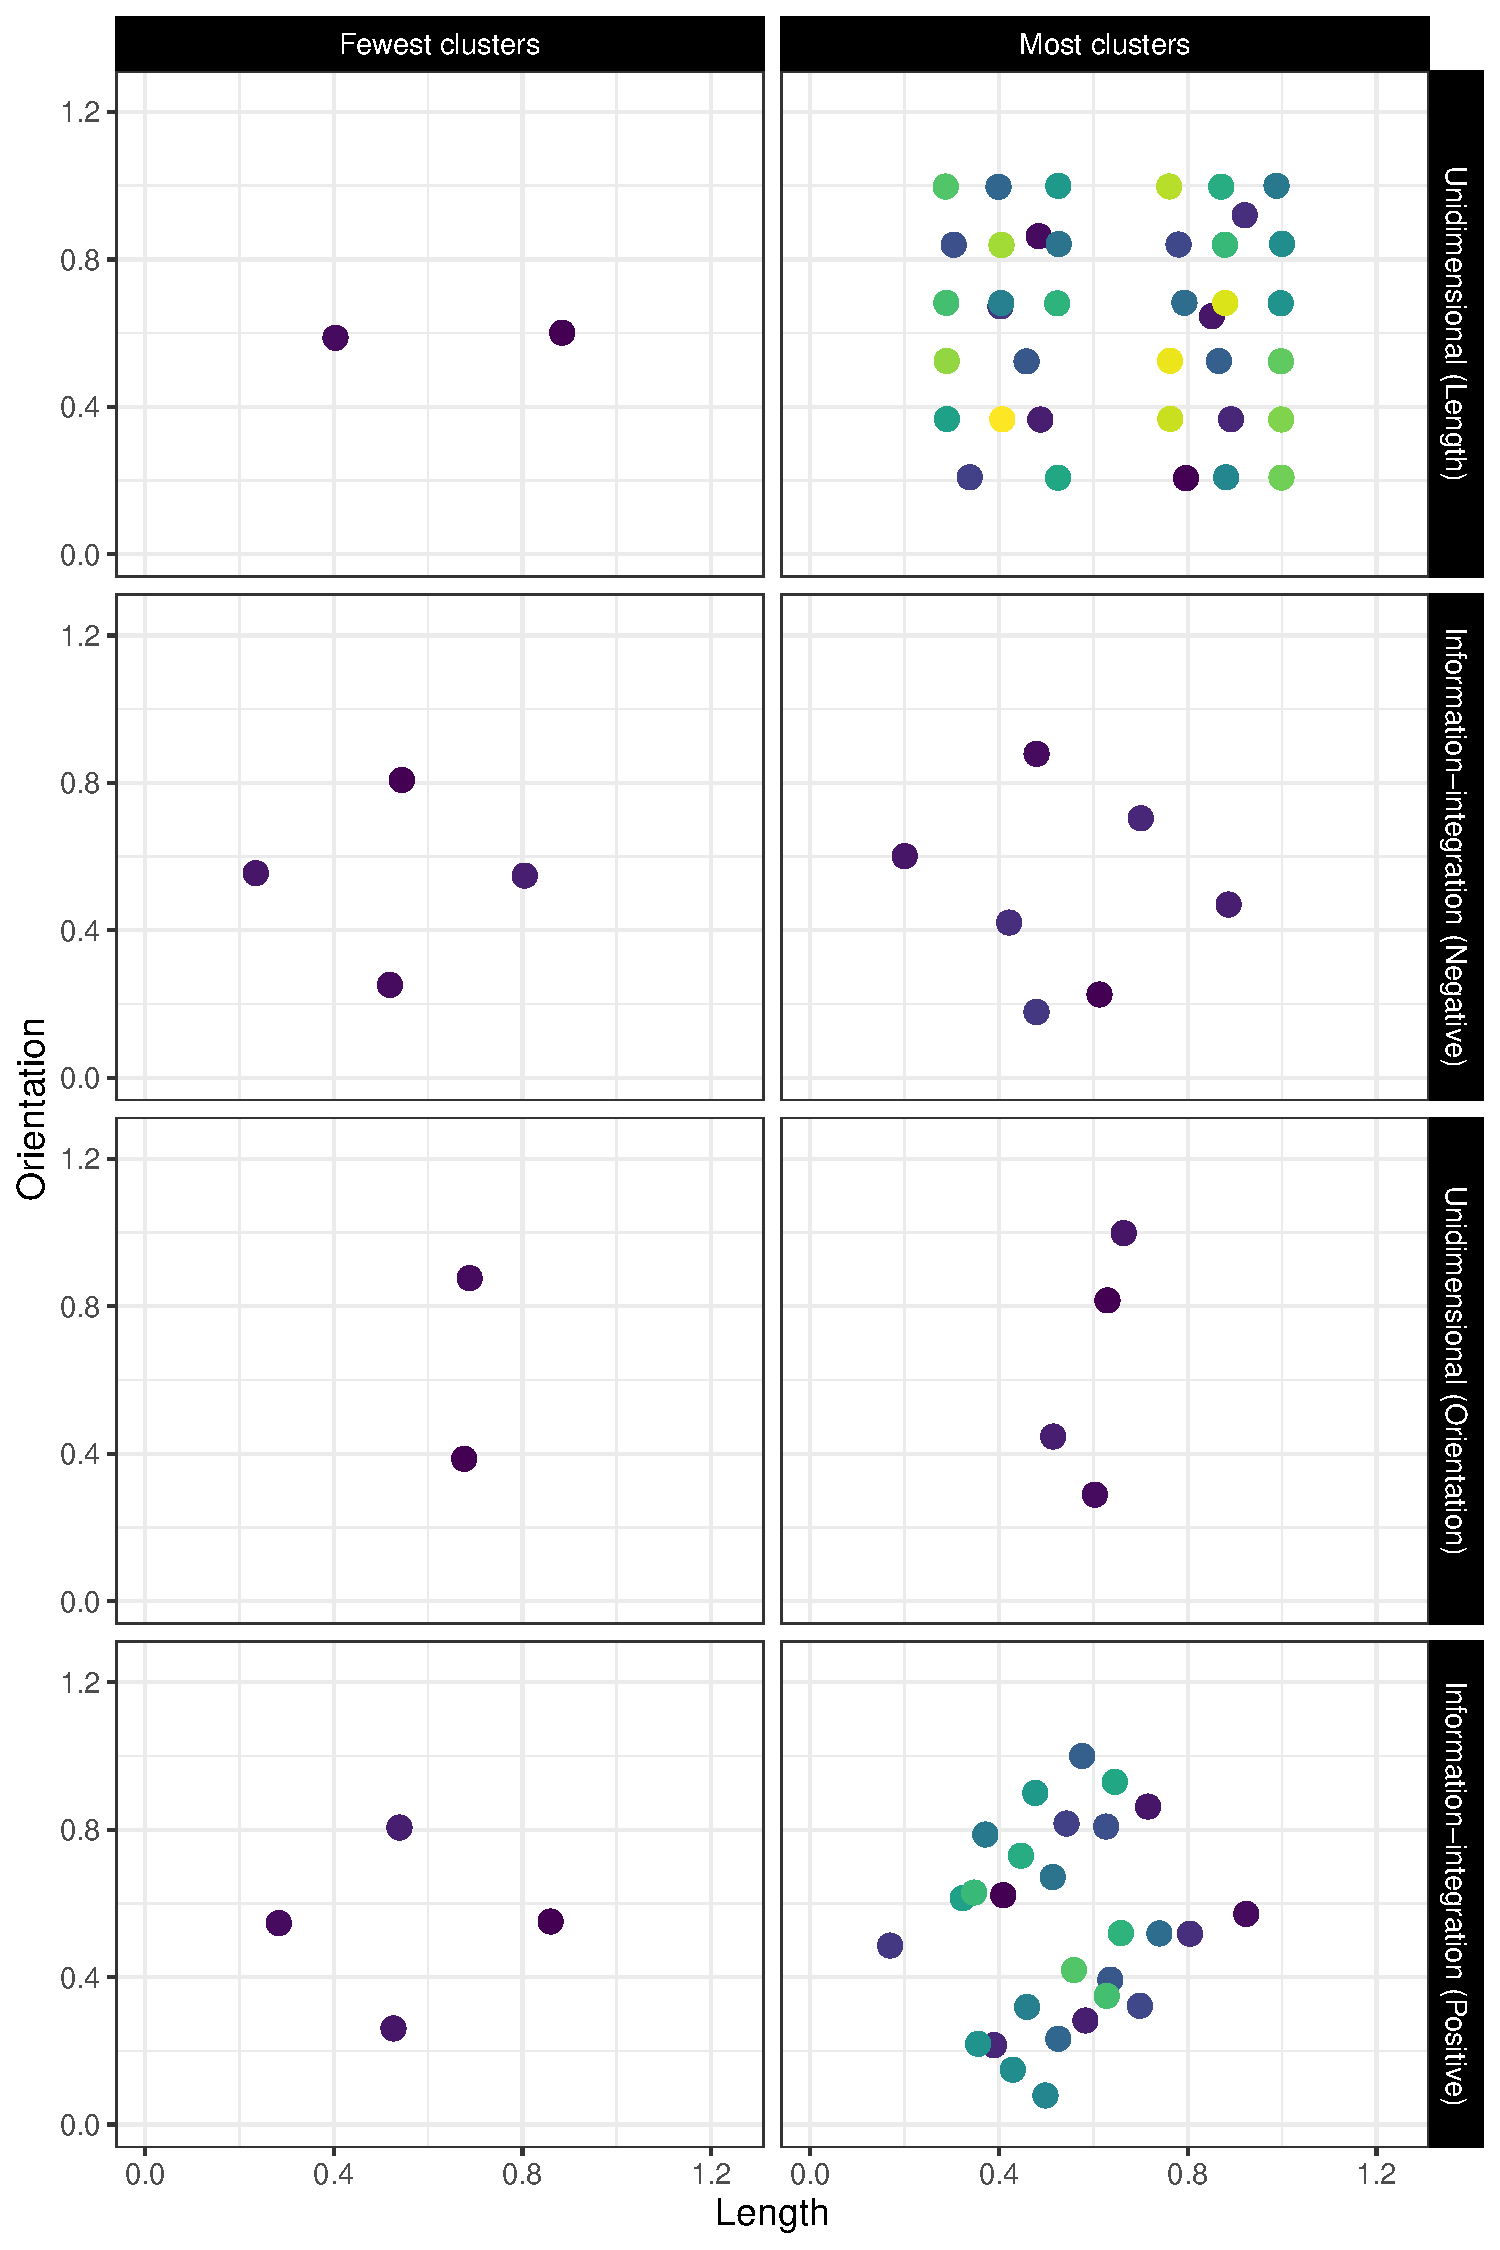
\includegraphics[width=0.8\textwidth]{Images/pu037clustersSUSTAIN}	
	\caption{Example clusters predicted from SUSTAIN. Each coloured dot represents a different cluster.}
	\label{fig:SUSTAINclusters}
\end{figure}

Further, our Recognition Entropy measure predicts that overall mean recognition memory
should be higher following II learning than UD, but the Recognition Score
predicts more comparable recognition memory, see Table~\ref{table:recognitionSUSTAIN}.
Recognition Scores tend to overlap between UD and II conditions, see 
Figure~\ref{fig:SUSTAINrecognition}. These scores can also become higher
for small number of clusters than high number of clusters. These issues
are not present with Recognition Entropy. Interestingly, both scores pedict
very high recognition memory for the extreme case, when SUSTAIN recruited
more clusters than stimuli.

\begin{table}[ht]
    \centering
\caption{Mean and standard deviation of the `Recognition Entropy' 
         and `Recognition Score` output from SUSTAIN} 
\label{table:recognitionSUSTAIN}
    \begin{tabular}{crlrrrr}  
        \hline
        & & \multicolumn{2}{c}{Entropy} & \multicolumn{2}{c}{Score}\\
        & Condition & Mean & SD & Mean & SD\\ 
    \hline
        UD & Length & 0.40 & 0.14 & 0.71 & 0.05\\ 
           & Orientation & 0.50 & 0.38 & 0.66 & 0.03\\ 
        II & Positive & 1.83 & 0.33 & 0.77 & 0.05 \\ 
           & Negative & 1.44 & 0.12 & 0.71 & 0.01 \\
    \hline
    \end{tabular}
    \end{table}



\begin{figure}
	\centering
	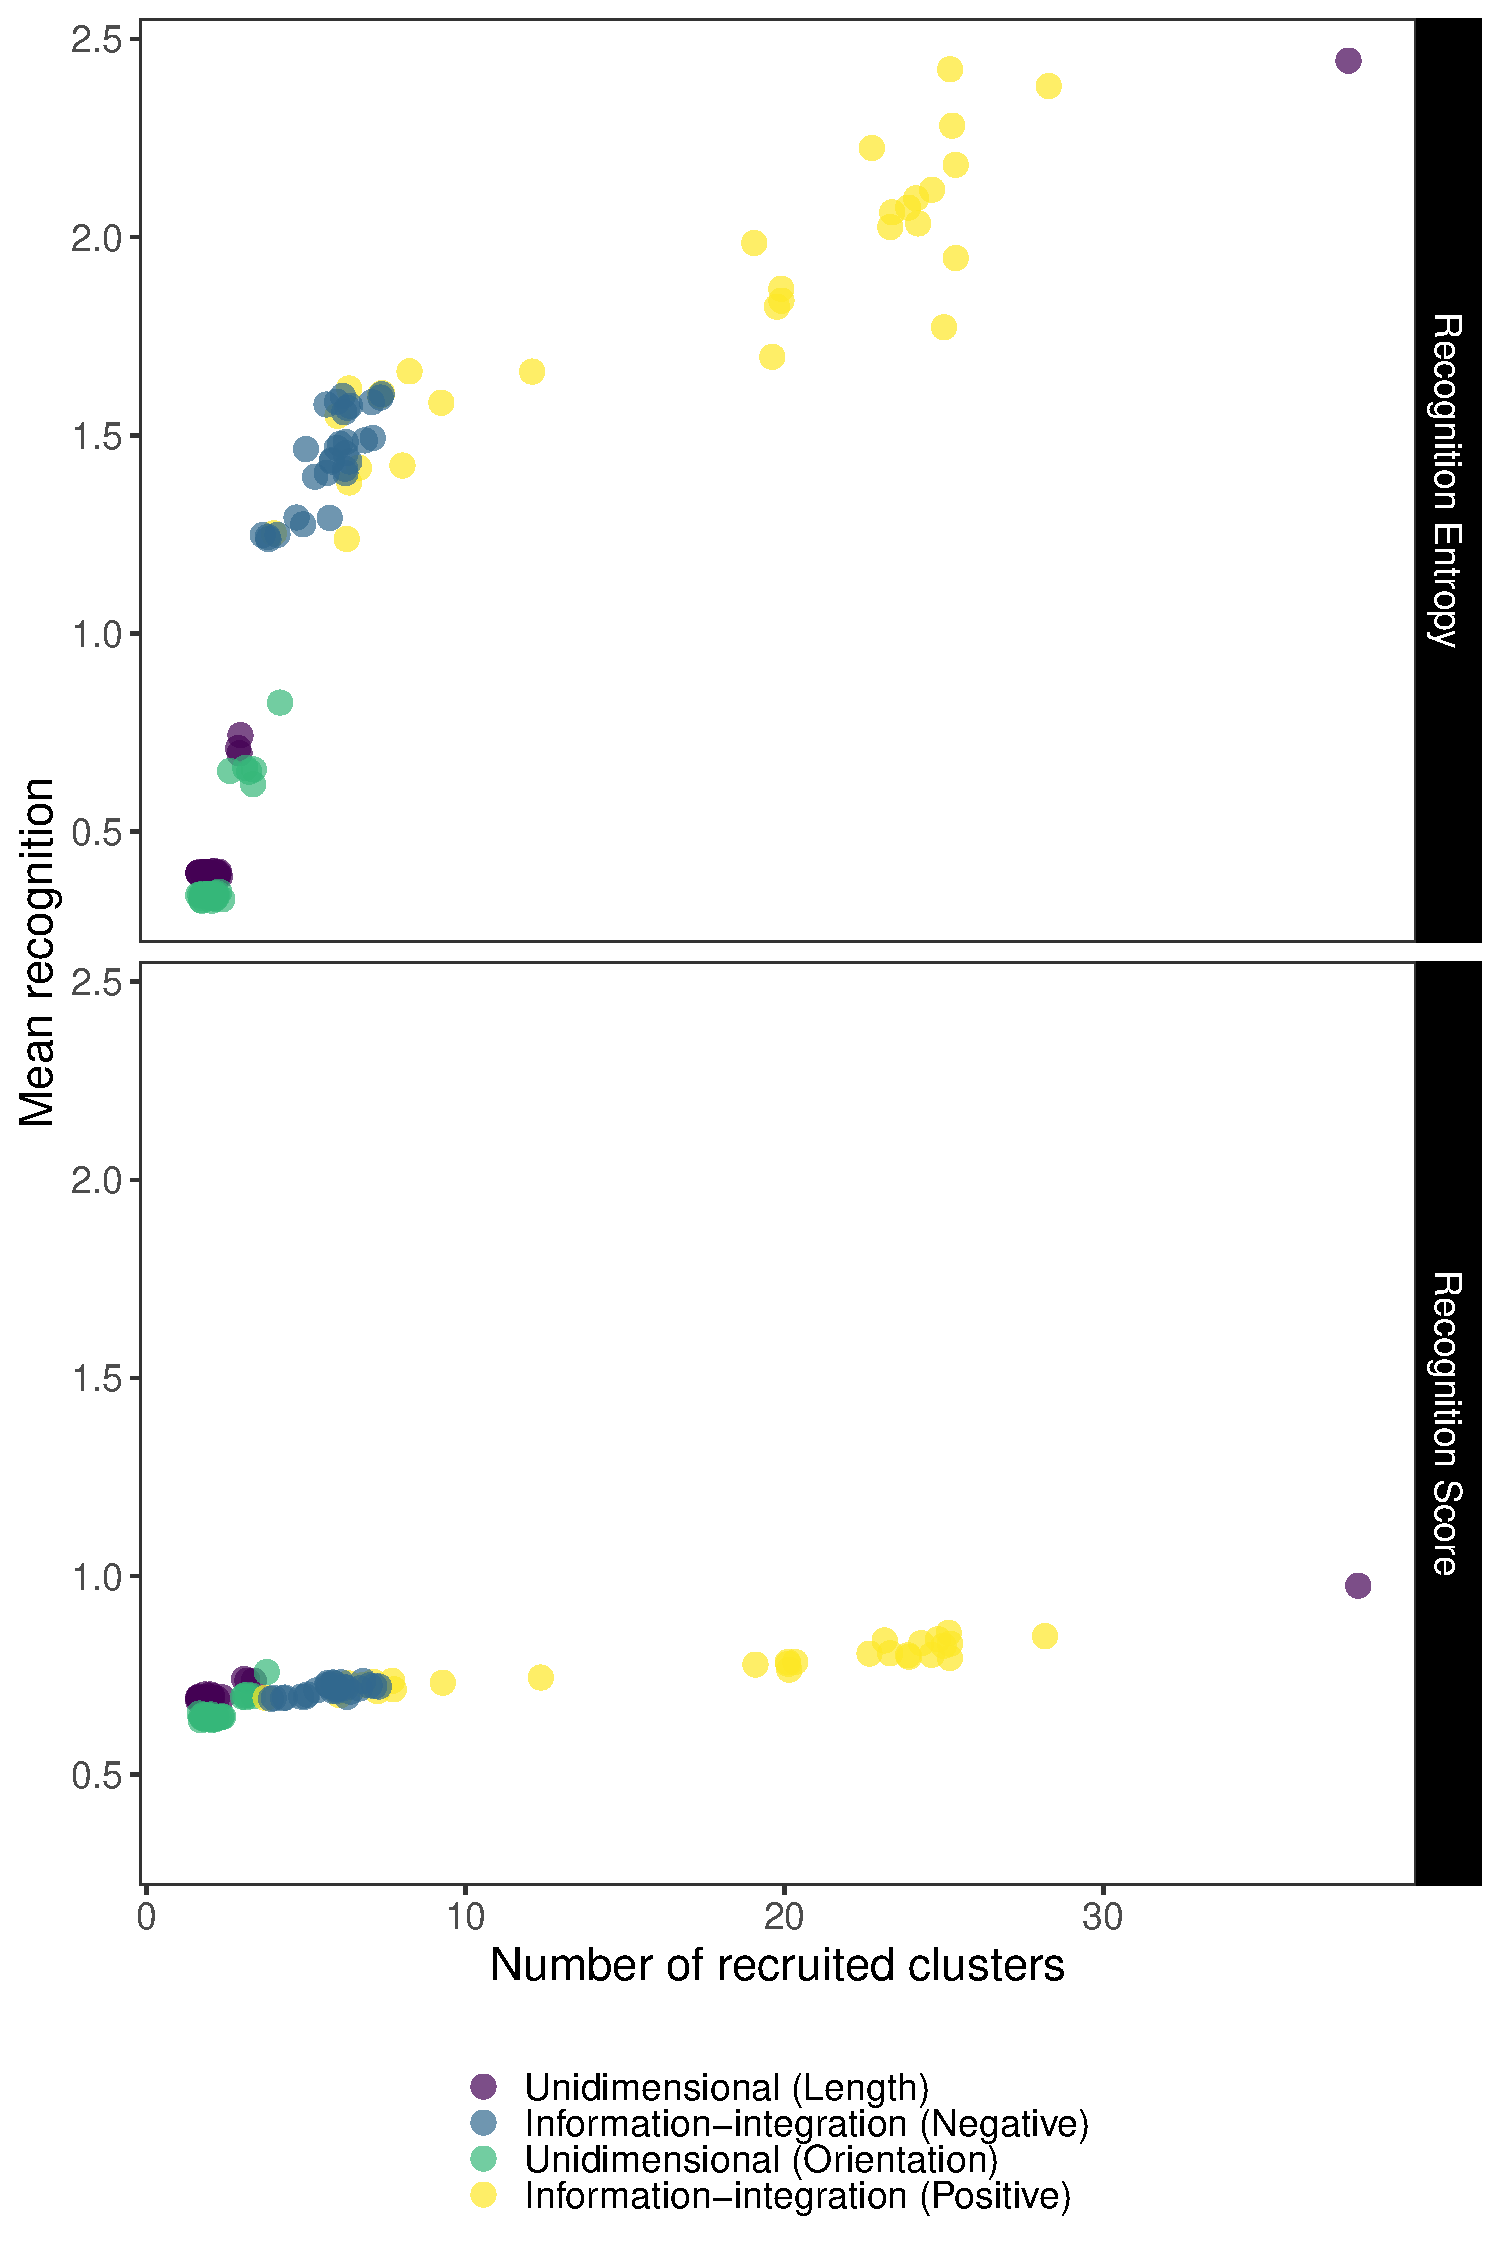
\includegraphics[width=0.8\textwidth]{Images/pu037recognitionGraph}	
	\caption{Example recognition performance for our Recognition Entropy
    and Recognition Score. Each coloured dot represents 
    a mean recognition performance for a simulated participant.}
    \label{fig:SUSTAINrecognition}
\end{figure}


\subsection{Conclusions from modelling}
% CE: This still needs to be edited. 
So, we can see here that SUSTAIN can learn information-integration category structures at least as well as researchers have found participants can in the literature. This suggests that, contrary to the intuitive predictions of those that promote the model, SUSTAIN can indeed learn the II task. 

However, along with that comes an additional prediction: SUSTAIN and our Recognition Entropy measure predicts that there should be higher recognition memory for items following learning the II task compared to those learning the UD task. This is contrary to the predictions of those who most frequently use II tasks as they would predict that participants learn this task procedurally, and therefore, that there would be poorer recognition memory following II learning than UD learning.

In summary, SUSTAIN predicts that a) it is possible to learn II tasks explicitly and b) that recognition performance following that will be higher after II than UD tasks. Therefore, in the following experimental work, we looked to see whether participants a) could report the strategy they used in training and b) whether they had higher recognition performance following II learning than UD learning. 

\section{Experimental work}
Here we report the combined estimates from four experiments. This was necessary given that the effect we expected to find was very small. This was due to a) the predicted difference by SUSTAIN and b) because the stimuli in perceptual categorization experiments tend to be very similar and thus, very confusable. In these four experiments, we attempted to make the stimuli more distinct whilst still maintaining their consistency with the previous literature. This was not successful (see Appendices for results from individual experiments), hence combining the information from all particiants across the four experiments using hierarchical Bayesian techniques. 

\subsection{Participants}
The participants were 155 undergraduate psychology students recruited from the Plymouth University participation pool. They were compensated with partial course credit for their participation.

\subsection{Category structures and stimuli}
The abstract category structures were identical in all these experiments. Half the participants were randomly assigned to learn a unidimensional rule-based category structure and the other half to learn an information-integration category structure (see Figure~\ref{fig:categoryStructures}).  The orientation of the category boundaries in abstract stimulus space were counterbalanced within conditions resulting in two unidimensional category structures--where the optimum boundary was vertical or horizontal--and two information-integration category structures--where the optimum boundary had either a positive or negative gradient.

These category structures were an adaption of the positive information-integration category structure used in Experiment~1 of \citeA{Spiering2008a}. To create the positive information-integration category structure, we added an additional row of 6 stimuli that were perpendicular to the category boundary. This brought the total number of stimuli up to 36, which facilitated the random selection of a third of stimuli as ``new'' items for the recognition task. The remaining category structures were rotations ($\pi/4$, $\pi/2$, $3\pi/4$ radians) of this adapted structure such that `centre of gravity' (i.e. the mean of both stimulus dimensions) of the points remained the same. The abstract stimuli coordinates were log-scaled so that all adjacent stimuli were approximately equally perceptually discriminable.

The stimuli varied between experiments, please see Appendices for detailed specifications. Experiment~1 used ; Experiment~2 used ; Experiment~3 used ; and Experiment 4 used. 

\subsection{Procedure}
The experiment was split into four phases: category training, recognition test, category test and verbal report questionnaire.

\paragraph{Category training.} First, participants were trained on two thirds
of the available stimuli. These training stimuli were selected randomly for
each participant subject to several constraints: 1) that those stimuli selected
were symmetrical around the category boundary and 2) that no adjacent stimuli
of similar difficulty were removed (for an example see
Figure~\ref{fig:categoryStructures}).  In total there were 360 training trials, split
into 3 blocks of 120 trials.  In each block, 24 stimuli were each shown 5 times
in a random order.  On each trial, the participants looked at the stimulus
until they made a response using either the ``Z'' key for Category A or the
``/'' key for Category B.  Participants were unable to respond until at least
500ms had passed. Following their response, either ``Correct'' in green or ``Incorrect!'' in red
was displayed for 500ms.  A blank white screen was displayed between each trial
for 500ms.  Throughout the experiment, the labels ``Category A'' and ``Category
B'' were displayed on the bottom left and right of the screen respectively.  If
participants took longer than 5000ms to respond, no corrective feedback was
given, instead the message ``PLEASE RESPOND FASTER'' was displayed for 500ms.

\paragraph{Recognition test.} Second, participants judged whether each stimulus
was ``old'' and appeared in the training phase, by pressing the ``O'' key, or
was ``new'' and had not been shown in the training phase, by pressing the ``N''
key.  The words ``New'' and ``Old'' were presented on the bottom left and right
of the screen respectively.  After this, participants judged the confidence
they had in their old-new judgement on a Likert scale that varied from 1
(=guessed) to 5 (=certain) by pressing the corresponding number key.  Following previous work \cite{Palmeri1995}, each of
the 36 stimuli were presented three times in a randomised order.  No feedback
was given.

\paragraph{Category test.} Third, participants were asked to judge the
category membership of all 36 stimuli, not just those they had seen in the
category training phase.  No corrective feedback was given in this phase.
Otherwise, the procedure was identical to that of the training phase.  Each of
the 36 stimuli were presented three times in a random order.

%\paragraph{Verbal report questionnaire.} Finally,
%participants were asked to complete a questionnaire that asked them to describe
%in detail the strategy that they used.  This was to determine whether the
%participants could explicitly report the strategy they used.
%The questionnaire asked them to ``Imagine that another participant was asked to complete the experiment as you did. What instructions would you give them so that they could exactly copy your pattern of responding?''  Participants were given a large blank box in
%which to write their answer.

\subsection{Analysis}
All analyses were conducting using R \cite{Rcore}. The trial-level raw data, verbal reports and analyses are available at \texttt{www.willslab.org.uk/pu037} with mds checksum \texttt{MDS checksum}. 

\subsection{Results} \label{section:results}
Three participants (two from the unidimensional condition, one from the information-integration) were removed because they failed to score over 50\% on the final categorisation test leaving 75 and 77 participants in the unidimensional and information-integration conditions respectively. 

Recognition performance was estimated using adjusted d-prime $d_a$, as the estimates of d-prime varied across confidence rating levels \cite{Macmillan2005}. This is calculated as follows
\begin{equation}\label{eqn:d_a}
	d_a = \left( \frac{2}{1+s^2} \right)^\frac{1}{2} \left[ z(H) - s z(F) \right]
\end{equation}
where $s$ is the slope of the receiver operating characteristic (ROC) curve, $H$ is the hit rate and $F$ is the false alarm rate. We also calculated the adjusted bias rate $c_a$ as follows
\begin{equation}\label{eqn:c_a}
c_a = \left( \frac{-\sqrt{2}s}{(1+s^2)^\frac{1}{2}(1+s)} \right) \left[ z(H) + z(F) \right]
\end{equation}
% How do you calculate s?

To determine whether information-integration training resulted in superior recognition memory than rule-based training, we estimated a Bayes Factor using hierarchical Bayesian estimation techniques \cite{Kruschke2015, Rouder:2018cz}. A Bayesian approach is ideal here for two reasons. First, it allows us to combine data from several experiments in a principled way \cite{Kruschke2015}. Second, unlike null-hypothesis significance testing, it allows us to find evidence for the null \cite{Dienes2011}. 

Our hierarchical model was specified as follows and is displayed graphically in Figure~\ref{fig:BayesianModel}. For both category structure conditions, the data ($d_{UD,i}$ and $d_{II,j}$) were assumed to be drawn from group-level Normal distributions. Denoting the grand mean by $\mu$, and the group difference in means by $\alpha$ and the group-level standard deviation by $\sigma$, the group-level Normal distribution for the unidimensional condition is defined as $N(\mu-\alpha/2, \sigma^2)$ and for the information-integration condition is defined as $N(\mu+\alpha/2, \sigma^2)$.

\begin{figure}
  \begin{minipage}{0.4\textwidth}
  \tikz[scale=1.5, every node/.style={scale=1.5}]{ 
  	\node[obs, minimum size=28pt] (UD) {$d_{UD,i}$};
    \node[obs, right=2.57cm of UD, minimum size=28pt] (II) {$d_{II,j}$}; 
    \node[latent, above=2.25cm of UD, minimum size=28pt] (mu) {$\mu$};
    \node[latent, above=2.25cm of II, minimum size=28pt] (sigma) {$\sigma$};
    \node[latent, right=0.46cm of mu, scale=1.1, minimum size=28pt] (alpha1) {$\alpha$};
    \node[latent, right=0.53cm of mu, minimum size=28pt] (alpha) {$\alpha$};
    \node[latent, above=of alpha, minimum size=28pt] (delta) {$\delta$};
	\edge {mu} {UD};
	\edge {mu} {II};
	\edge {sigma} {UD};
	\edge {sigma} {II};
	\edge {sigma} {alpha1};
	\edge {delta} {alpha1};
	\edge {alpha1} {UD};
	\edge {alpha1} {II}; 
	\plate[inner sep=-0.2cm, scale=0.85] {plateUD} {(UD)} {\tiny $i=1,\dots,75$};
	\plate[inner sep=-0.2cm, scale=0.85] {plateII} {(II)} {\tiny $j=1,\dots,77$};
  }
  \end{minipage}
  \begin{minipage}{0.1\textwidth}
  	\hspace{1cm}
  \end{minipage}
  \begin{minipage}{0.4\textwidth}
  	$\theta_{UD, i} \sim Normal(\mu-\alpha/2, \sigma^2)$
  	
  	\vspace{20pt} 
  	
  	$\theta_{II, j} \sim Normal(\mu+\alpha/2, \sigma^2)$	
  	
  	\vspace{20pt}
  	$\mu \sim Normal(0, 1)$
  	
  	$\sigma \sim Uniform(0, 5)$
  	
  	$\alpha = \delta * \sigma$
  	
  	$\delta \sim M*slab + (1-M)*slab$
  	
  	$slab \sim Normal(0.3, 0.15)$
  	
  	$spike \sim Normal(0, 1x10^{-5})$
  	
  	
  \end{minipage}
  \caption{Graphical representation of the model used to estimate Bayes Factor.}
  \label{fig:BayesianModel}
\end{figure}

For the parameters that are not subject to statistical test (i.e., $\mu$ and $sigma$) we specified uninformative priors. The prior for the group mean $\mu$ was the standard Normal and for $sigma$ was a uniform distribution between 0 and 5. The key aspect of our model is the parameter $\delta$ that quantifies effect size, $\delta=\alpha/\sigma$. This means that positive $\delta$ represents an effect of information-integration training resulting in greater memory than rule-based training, with negative $\delta$ indicating the opposite. We used the spike-and-slab prior on $delta$ \cite{Rouder:2018cz}. A spike-and-slab prior is a mixture of a null model (the \emph{spike}) and an effect model (the \emph{slab}).  The spike was represented a Normal distribution, with mean 0 and a standard deviation of $1 \times 10^{-3}$. The slab was distributed as a Normal distribution, with mean 0.3 and standard deviation 0.15, representing a small effect size greater than zero \cite{Dienes2011}. The spike model was weighted as 0.9 and the slab model as 0.1, as previous runs indicated a bias towards sampling from the slab model \cite{Kruschke2015}.

We drew MCMC samples from the posterior distribution for $\delta$, we ran 4 chains for 50000 iterations each, discarding the first 1000 trials as burn-in. We visually inspected the chains and calculated the \citeA{Gelman:1992ht} {\it \^{R}} statistic to check that the chains had converged. When the posterior was compared to the prior, this resulted in a Bayes Factor of $B_{10}=12.02$. This provides positive support for better recognition performance post information-integration training than after rule-based training, compared to the null. 

\section{General Discussion}
The SUSTAIN model has been successful in accounting for many categorization effects \cite{Love2004}. 
However, proponents of the SUSTAIN model put procedural learning well outside its explanatory domain \cite{Davis2012a}. 
Further, \citeA{Davis2012a} did not directly test whether or not this was the case. 
Therefore, in the current paper, we more carefully investigated whether the SUSTAIN model could account for the patterns of learning in a task argued to be learned procedurally \cite{Ashby:2017fm}. 

By fitting the formal model to the category structure, we showed that SUSTAIN could learn an II category structure at least as well as found in the literature. 
We further used this model fitting to make predictions that could discriminate between SUSTAIN and a procedural learning account. 
We found superior recognition performance following the II task than the UD task. 
This is consistent with the predictions of the SUSTAIN model, but not consistent with the assumption that participants learning II category structures procedurally. 

\subsection{Resolving the conflict with the literature}
So, if our results fail to find evidence of procedural learning during an II task, why are II tasks widely argued to be learned procedurally?
Part of the reason may perhaps be because reviews of the literature can be biased \cite{Wills2019}. 
In actuality, there is a great deal of experimental and modelling literature that casts doubt on whether II tasks are learned procedurally. 

First, many of the experiments that showed learning to affected in a way that was consistent with procedural learning, have been re-interpreted by other, subsequent work. 
For instance, in our lab we re-examined work that showed poor learning of II tasks with an observational procedure \cite{Ashby2002a}. 
We found that performance in the II task was very similar to another, rule-based, two-dimensional categorization task. 
Therefore, it appears that the previous dissociation might be better understood as a dissociation between the number of relevant stimulus dimensions for categorization, rather than between a rule-based and procedural learning mechanism. 

Further, participants learning II tasks are well able to describe the strategies they used to complete the task. 
In several of our previous experiments, we have asked participants to describe the strategies they used to complete the learning task \cite{Edmunds2015, Edmunds2017}[ANALOGICAL TRANSFER]. 
Participants who learned an II task tend to report using a two-dimensional, rule-based strategy rather than reports that would be consistent with procedural learning such as an overall similarity strategy or going with their gut. 

Finally, another key assumption in this literature has shown to be flawed. 
Experiments using an II task often use a decision-bound strategy analysis to check that participants are learning the category structures optimally. 
In this approach, evidence that participants learned the task procedurally comes from the fact that participants appeared to use the optimum strategy for the task. 
However, this argument is rather circular: II tasks are learned procedurally, the participants learned the task using the optimum solution, therefore they learned the task procedurally. 

Unfortunately, this approach has been shown to be unreliable \cite{Donkin2015, Edmunds2018}. 
In decision-bound modelling, strategies are determined by fitting several different strategies to the responses from each participant. 
Then, a participant's strategy is argued to be the one that best fits. 
However, the evidence suggests that successful recovery of the correct strategy depends on whether you include the correct strategy in the set \cite{Donkin2015, Edmunds2018} and the category structure under consideration. 
Most importantly, the analysis is biased towards finding that participants used the optimal strategy for the category structure, no matter which strategy they actually used. 
Indeed, we were able to apparently recover that participants used the optimal strategies but were simulated as using rule-based strategies, at the same level of accuracy in published work \cite{Edmunds2018, Smith2014}.
This suggests that many of the participants that were argued to learn procedurally using this approach could have been using multi-dimensional rule-based strategies. 
Indeed, this would be more consistent with the reports that participants have given \cite{Edmunds2015, Edmunds2017}[ANALOGICAL TRANSFER]. 
Thus, it seems like there is much evidence that suggests that II tasks are not learned procedurally. 

\subsection{Conclusion}
Here, we investigated the predictions of the SUSTAIN model of category learning \cite{Love2004}. 
Contrary to a prior claim, we found that SUSTAIN can account for learning of II category structures. 
Further, we argue that this adds to evidence that II category structures are not learned procedurally. 

\subsection{Open practices statements}
All data and analysis code is available in the Open Sciences Framework at \url{www.osf.com/}. 

\subsection{Author contributions}
C. E. R. Edmunds ran the experiments, analyzed them, aided in the modelling and took the lead on writing the paper. 
Lenard Dome finalised the modelling and wrote the modelling section. 
Fraser Milton advised on experimental design and provided valuable insight on analysis and the paper. 
Andy J. Wills advised as his rule as Ph.D. supervisor of C. E. R. Edmunds and Lenard Dome.  

\newpage
\bibliographystyle{apacite}
\bibliography{References}

\newpage
%\section{Appendix}
%\subsection{SUSTAIN modelling}
%
%\subsection{Experiment 1}
%\subsubsection{Stimuli}
%The stimuli were 36 grey squares that varied in brightness and size displayed
%on a white background. The abstract and logged scaled stimulus coordinates are archived along with the raw data at \url{www.willslab.org.uk/ply40}.
%
%\subsubsection{Results}
%A t-test found that recognition performance in the information-integration
%condition was significantly different from chance, ${d_a=0.13}$, ${SD=0.21}$,
%${t(20)=2.80}$, ${p=.011}$.  Additionally, the difference between performance
%in the unidimensional condition and chance failed to reach significance,
%${d_a=0.09}$, ${SD=0.27}$, ${t(20)=1.58}$, ${p=.129}$.  However, the difference
%between recognition memory performance between the unidimensional and
%information-integration category structure conditions failed to reach
%significance, ${t(40)=0.51}$, ${d=0.16}$, ${p=.615}$.  There were also no
%significance differences in response bias between the unidimensional and
%information-integration category structure conditions, ${t(40)=1.00}$,
%${d=0.31}$, ${p=.323}$.
%
%\begin{figure}[!b]
%\centering
%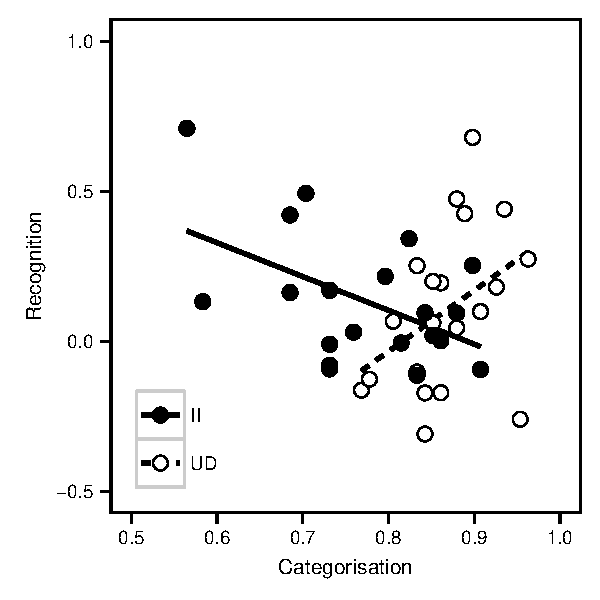
\includegraphics[width=0.5\textwidth]{Images/PLY40graphCorrelation}
%\caption[The relationship between categorisation accuracy and recognition in
%\nameref{exp:PLY40}]{The relationship between categorisation accuracy and
%recognition in \nameref{exp:PLY40}. Each point represents a participant, each
%line the line of best fit for each condition. Conditions:
%II=Information-integration, UD=Unidimensional.}
%\label{graph:PLY40cor}
%\end{figure}
%
%It may also be informative to look at the relationship between categorisation
%and recognition performance.  COVIS would predict that good performance on the
%information-integration category learning task is due to participants switching
%from the explicit, Verbal System to the implicit, Procedural System.
%Therefore, it would predict that as performance on the information-integration
%categorisation task improves, recognition performance should decrease.
%Whereas, all participants in the rule-based categorisation task should have
%high recognition performance as they are using the Verbal System.
%
%My predictions were based on the assumption that participants who learn the
%information-integration category structure well use complex, rule-based
%strategies.  Therefore, one might expect that participants who perform better
%on the categorisation task use more complex strategies and so may also perform
%better on the recognition task.  Whereas, good performance on the
%unidimensional categorisation task is unlikely to be correlated with
%recognition performance as all the participants will use the same, simple
%strategy.  Therefore, we might expect that participants in the rule-based
%condition would all have poor recognition performance.
%
%An ANCOVA found a significant interaction between category structure conditions
%and the relationship between category learning performance and recognition,
%$F(1,37)=8.34$, $p=.004$.  This interaction was driven by participants in the
%information-integration condition, $F(1,19)=6.61$, $R^2=0.26$, $p=.019$.
%Recognition performance could be predicted from categorisation performance
%according the formula: recognition = 1.00 - 1.13*categorisation.  For the
%rule-based condition this relationship did not reach significance, $F(1,
%18)=3.43$, $R^2=0.16$, $p=.081$.
%
%\subsubsection{Materials}
%The experiment was run using MATLAB with the Psychophysics Toolbox
%\cite{Brainard1997, Pelli1997} extensions on a desktop computer with a
%21.5-inch screen.
%
%\subsection{Experiment 2}
%\subsubsection{Stimuli}
%The abstract and logged scaled stimulus coordinates are archived along with the raw data at \url{www.willslab.org.uk/ply51}.
%
%
%\subsection{Experiment 3}
%\subsubsection{Stimuli}
%The abstract and logged scaled stimulus coordinates are archived along with the raw data at \url{www.willslab.org.uk/ply76}.
%
%\subsection{Experiment 4}
%\subsubsection{Stimuli}
%The abstract and logged scaled stimulus coordinates are archived along with the raw data at \url{www.willslab.org.uk/ply87}.
%
%\section{Supplementary Material}
%\subsection{Model-based strategy analysis}
%It is possible that category learning is mediated by dual-systems of learning, but that the majority of participants in these experiments did not switch to the optimum system for the category structure.  If this was the case, failing to find a dissociation would be predicted by the COVIS model.
%
%This is a valid criticism due to the logic of COVIS experiments \cite{Ashby2011b}.  COVIS predicts that there are two learning systems that mediate different kinds of learning strategy: rule-based and information-integration \cite{Ashby1998, Ashby2011c}.  Therefore, because these systems implement different strategies, the systems will be able to optimally learn different types of category structure.  However, the experimental evidence that supports COVIS uses this information the other way around.  In the majority of COVIS experiments, the experimenters manipulate the category structure hoping that participants will use the strategies, and thus the system, that is most appropriate to that category structure.  However, there is always the possibility that when learning an information-integration category structure participants fail to switch from the Verbal System to the Procedural System.
%
%To overcome this objection, experimental work within the COVIS literature uses a model-based strategy analysis to determine which strategy the participant is using \cite<e.g.>{Maddox2003}.  This strategy analysis is based on General Recognition Theory \cite<GRT;>{Ashby1988} and is a multi-dimensional generalisation of Signal Detection Theory \cite{Macmillan2005}.  For each participant, this analysis determines the optimum decision boundary in stimulus space that separates the stimuli judged by each participant to be in Category A from those in Category B.  Each participant is then assigned a strategy type on the basis of characteristics of their optimum boundary.  Typically, it is assumed that the category type manipulation has successfully resulted in a change of category learning system if more participants are using the optimum decision bound model for the category structure they have been assigned to than are using a sub-optimum strategy.  Although it is important to note that this criterion can be flexible \cite<see>[for an example of an alternative criterion]{Smith2015a}.
%
%The GRT-based analysis determines which of a set of experimenter-selected decision-bound models best describes the pattern of responding for each participant \cite{Maddox1993}.  Although this analysis is ubiquitous in the experimental COVIS literature, the types of strategy models included, and their precise specifications, often vary between applications of this analysis (see Chapter~\ref{chapter:grt} for more discussion of the effects of this).  Therefore, to facilitate comparison with the analysis presented in \citeA{Spiering2008a}, here we will use the analysis as reported in that paper.
%
%As in Chapter~\ref{chapter:feedbacktype}, the set of models considered by \citeA{Spiering2008a} included three main types: rule-based, information-integration and random models.   Within the COVIS framework, the unidimensional and conjunction models are considered to represent explicit, rule-based strategies, while the diagonal (GLC) strategy is considered to represent an implicit, information-integration strategy.   Therefore, in these experiments the category structure manipulation will be considered successful if more participants are found to be using the diagonal strategy than a rule-based strategy (either unidimensional or conjunction).
%
%The strategy models used in this analysis were specified as follows:
%
%\paragraph{Unidimensional models.} These assume that the participant determines a criterion along one of the stimulus dimensions, either orientation or length.  They then make a decision about the category membership of each stimulus by comparing the appropriate stimulus attribute with the criterion value.  As an example, for length, this corresponds to a rule of the type: `Assign to Category A if the stimulus is long, or Category B if short'.  The unidimensional models have two parameters: the value of the criterion and the variance of internal (criterial and perceptual) noise.
%
%\paragraph{Conjunction models.} These assume that the participants make two judgements, one for each stimulus dimension, and then combine these to make a judgement about category membership.  The conjunction rule in the current analysis was of the type: `Assign to Category A if the stimulus is short and upright, otherwise assign to Category B'.  The conjunction model had three parameters: the two criterion values and internal noise.
%
%\paragraph{General linear classifier (GLC) models.} These assume that the decision boundary between the categories can be described by a straight line that can vary in gradient and intercept.  The unidimensional models are therefore special cases of the GLC model.  The GLC model has three parameters: the intercept and slope of the decision bound, plus noise.
%
%\paragraph{Random models.} These assume that participants are responding randomly.  The \emph{random} model assumes that participants have no preference for either category: it has no parameters.  The \emph{random bias} model assumes that participants respond randomly but prefer one category over the other.  It has one parameter that represents the amount of bias.
%
%For each participant, the fit of each of these models was calculated using the Bayesian Information Criterion \cite<BIC;>{Schwarz1978}
%
%\begin{equation}
%BIC = r \ln N - 2 \ln L
%\end{equation}
%
%where $r$ is the number of parameters in the model, $N$ is the sample size and $L$ is the likelihood of the model given the data.  The results from this analysis, which was performed using the \texttt{grt} package in the R environment \cite{Matsuki2014}, are reported in Table \ref{table:TOgrt}.
%
%\begin{table}[!]
%\centering
%\caption{The proportion of participants in each experiment of that were identified as using each strategy
%type using the model-based analysis.}
%\renewcommand{\arraystretch}{1.25}
%\addtolength{\tabcolsep}{3pt}
%\begin{tabular}{l C{1.86cm}C{1.86cm}C{1.86cm}C{1.86cm}}
%\toprule
%\multirow{2}{3cm}{Category structure} & \multicolumn{4}{c}{Strategies {\it
%(wBIC)}}\\
%\cline{2-5}
% & UD & GLC & CJ & RND \\
%  \midrule
%Experiment 1 & & & & \\
%\IE Unidimensional & 0.81 {\it (0.78)}& 0.10 {\it (0.98)}& 0.05 {\it (0.58)}&
%0.05 {\it (0.69)}\\
%\IE Information-integration & 0.29 {\it (0.80)}& 0.57 {\it (0.97)}& 0.10 {\it
%(0.65)}& 0.05 {\it (0.44)}\\
%
%Experiment 2 & & & & \\
%\IE Unidimensional & 0.83 {\it (0.82)}& 0.12 {\it (0.84)}& 0.04 {\it (0.67)}& -
%\\
%\IE Information-integration & 0.20 {\it (0.72)}& 0.50 {\it (0.93)}& 0.15 {\it
%(0.66)}& 0.15 {\it (0.66)}\\
%
%Experiment 3 & & & & \\
%\IE Unidimensional & 0.75 {\it (0.81)}& 0.05 {\it (0.54)}& 0.20 {\it (0.75)}&
%-\\
%\IE Information-integration & 0.04 {\it (0.57)}& 0.92 {\it (0.91)}& 0.04 {\it
%(0.76)}& - \\
%
%Experiment 4 & & & & \\
%\IE Unidimensional & 0.80 {\it (0.79)}& 0.15 {\it (0.74)}& 0.05 {\it (1.00)}& -
%\\
%\IE Information-integration & - & 0.90 {\it (0.95)}& 0.10 {\it (0.86)}& - \\
%
%\bottomrule
%\multicolumn{5}{D{\textwidth}}{Strategies: UD=Unidimensional, GLC=General
%linear classifier, CJ=Conjunction, RND=Random.}
%\end{tabular}
%\label{table:gsrt}
%\end{table}
%
%As required by the COVIS model, the majority of participants in each condition
%are using the optimum strategy for the category structure they learned.  In
%other words, in the rule-based condition, more participants are using the
%unidimensional strategy than any of the other strategies.  Similarly, in the
%information-integration condition more participants are using the diagonal
%(GLC) strategy than any of the others.  This analysis (as used by the
%proponents of COVIS) indicates that the category structure manipulation
%resulted in a corresponding switch in learning system.

%That being said, I have serious reservations about the validity of this
%analysis.  For instance, in Chapters~\ref{chapter:feedbacktype} and
%\ref{chapter:difficulty}, across 5 experiments, the strategy analysis
%corresponded very poorly with the strategies that the participants described
%using.  This issue will be discussed in greater detail in
%Chapter~\ref{chapter:grt}.  For the present, the take away message is that
%these experiments meet the criteria typically used in the COVIS literature and
%therefore, the results of these experiments can be generalised to other
%experiments within this literature.

%In this section, we examine what the SUSTAIN model predicts regarding recognition performance following unidimensional and information-integration category learning. This model was made simple by the use of the \texttt{catlearn} package \cite{catlearn, Wills:2017ez} implemented using R \cite{Rcore}. Briefly, \texttt{catlearn} exemplifies the Open Models approach to conducting and sharing simulations with formal cognitive models by making code openly available. 
%
%What follows is a brief description of the mathematics of SUSTAIN, followed by details of the model fitting and simulations. For a detailed description of the model, please see \citeA{Love2004}. 
%
%SUSTAIN can be thought of in three stages: linking stimuli and clusters, decision-making and dealing with feedback. 
%
%\subsection{Linking stimuli and clusters}
%In SUSTAIN, category structures are represented by clusters of stimuli. Each cluster has a receptive field for each stimulus dimension. A stimulus activates a particular cluster to the extent that it is central in that cluster's receptive field. 
%
%Mathematically, the response $\alpha$ of the receptive field on a particular stimulus dimension is modeled as exponentially decreasing as the distance of the stimulus from the field's center increases
%\begin{equation}
%	\alpha(\mu) = \lambda_i \exp^{-\lambda_i\mu}	
%\end{equation}
%where $\mu$ is the absolute distance of the stimulus from the center of the field and $\lambda_i$ is the tuning of the receptive field on dimension $i$. Unlike the center of the receptive field, the tuning of the receptive field (i.e. how wide it is) is dimension specific and the same for all clusters. These tunings change throughout learning. Dimensions that are highly attended to develop peaked tunings, whereas those that are relatively unattended develop broader tunings. We assume that each dimension is given equal weight at the beginning of training (i.e. $\lambda=1$ for both dimensions).
%
%Then, the activation of a cluster is given by 
%\begin{equation}
%	H_j^\text{act} = \frac{\sum_{i=1}^m (\lambda_i)^r \exp(-\lambda_i\mu_{ij})}{\sum_{i=1}^m(\lambda_i)^r}
%\end{equation}
%where $H_j^\text{act}$ is the activation of the $j$th cluster, $m$ is the number of stimulus dimensions, $\lambda_i$ is the tuning for the $i$th input dimension and $r$ is the attentional parameter (always non-negative). If $r$ is set to zero, every dimension receives equal weighting. As $r$ increases, the dimensions that have the largest attention (i.e. largest attention) are weighted more and more. 
%
%Clusters compete to respond to stimuli. 
%
%For the winning cluster, with the greatest activation $H_j^\text{act}$:
%\begin{equation}
%	H_j^\text{out} = \frac{(H_j^\text{act})^\beta}{\sum_{i=1}^n (H_i^\text{act})^\beta} H_j^\text{act}	
%\end{equation}
%where $n$ is the number of clusters, and $\beta$ is the lateral inhibition parameter (always non-negative) that regulates cluster competition. When $\beta$ is large, the winner is only weakly inhibited. 
%
%For all other clusters, $H_j^\text{out}=0$. 
%
%\begin{equation}
%	C^\text{out}_{zk} = \sum_{j=1}^n w_{j, zk} H_j^\text{out}
%\end{equation}
%
%
%\subsection{Making a response}
%\begin{equation}
%	P(k) = \frac{\exp(d C^\text{out}_{zk})}{\sum_{j=1}^{v_z}\exp(d C^\text{out}_{zj})}	
%\end{equation}
%
%
%
%
%\subsection{Dealing with feedback}
%After responding, feedback is incorporated into SUSTAIN. The target value for the $k$th category unit of the queried dimension $z$, here the category label, is
%\begin{equation}
%	t_{zk} = 
%		\begin{cases}
%  			\max(C^\text{out}_{zk}, 1) \enspace \text{if} \enspace I^{\text{pos}_{zk}}=1\\    
%  			\min(C^\text{out}_{zk}, 0) \enspace \text{if} \enspace I^{\text{pos}_{zk}}=0.
%		\end{cases}
%\end{equation}
%
%If the winning cluster predicts an incorrect response, a new cluster is added. It is centered on the misclassified input pattern. Then, the clusters' activations and output are recalculated. 
%
%The position of the winning cluster is adjusted towards the stimulus according to
%\begin{equation}
%	\Delta H_j^{\text{pos}_{ik}} = \eta (I^{\text{pos}_{ik}} - H_j^{\text{pos}_{ik}})
%\end{equation}
%where $\eta$ is the learning rate. 
%
%Additionally, the tunings are adjusted according to 
%\begin{equation}
%	\Delta \lambda_i = \eta \exp(-\lambda_{i}\mu_{ij})(1-\lambda_i\mu_{ij})
%\end{equation}
%where $j$ 
%
%When a cluster is recruited, weights from the unit to the output units are zero. The weights are adjusted according to 
%\begin{equation}
%	\Delta w_{i, zk} = \eta(t_{zk} - C^\text{out}_{zk}) H^\text{out}_j
%\end{equation}
%where $z$ is the queried dimension. 



\end{document}

%%% Local Variables:
%%% mode: latex
%%% TeX-master: t
%%% End:
